% !TEX root = mythesis.tex

%==============================================================================
\chapter{Data and Monte Carlo simulated events}
\label{chap:data_MC}
%==============================================================================
\section{Data sample}
\label{sec:data_sample}

The analysis presented in this thesis uses data collected from 2015 to 2018 by the ATLAS detector at a center-of-mass energy of 13 TeV, The selected data periods were collected during stable beam LHC operations and with the ATLAS detector fully functioning. The total integrated luminosity is 139 fb$^{-1}$. Figure \ref{atlasluminosity} shows the total integrated luminosity over time. The considered data events have been recorded by either electron or muon trigger. There were later filtered using so-called the Good Run List (GRL), which requires that the LHC beam has conditions to qualify it for physics analysis and is is shown in blue in figure \ref{atlasluminosity}.

\begin{figure}[!h]
\centering
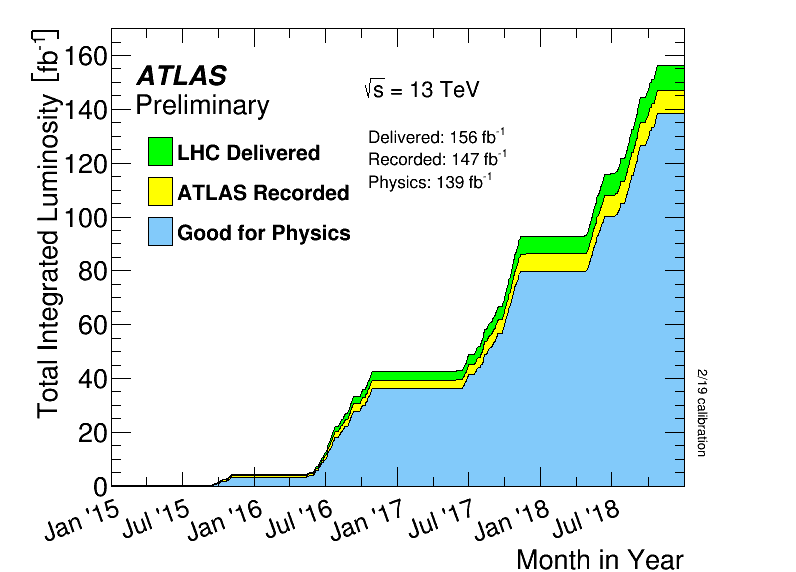
\includegraphics[width=0.7\textwidth]{ubonn-thesis/Chapters/Chapters_04/Figure/intlumivstimeRun2DQall.png}
\caption{Cumulative luminosity versus time delivered to ATLAS (green), recorded by ATLAS (yellow), and certified to be good quality data (blue) during stable beams for pp collisions at 13 TeV centre-of-mass energy in 2015-2018 \cite{ATLAS-CONF-2020-023}}
\label{atlasluminosity}
\end{figure}


\section{Monte Carlo simulation}
\label{sec:MC}
Monte-Carlo (MC) simulation is an inevitable component of the ATLAS experiment in order to simulate all physics processes considered in the analysis. Because MC events are used to validate the analysis procedures to calculate the acceptance for the signal channel and to evaluate the contributions from the background processes. The MC simulation is divided into three steps \cite{buckley2019monte}: The first is the detector independent generation of collision events which can be done by various extenal MC event generators interfaced by the ATLAS software framework Athena \cite{atlas_collaboration_2019_2641997} . The event generation of the MC simulation includes the parton shower and hadronization process. The nect step of the MC simulation is the detector simulation, where a realistic picture of the energy deposit in the sensitive parts of the detector is simulated. The GEANT4 \cite{GEANT4:2002zbu} toolkit is used to perform this simulation. It relies on the detector geometry, which describe physics constructions and conditions (e.g. magnetic field, alignment of detectors parts, dead read-out channels) of the detector. The last step of the MC simulation of all events is the digitization of the simulation hits. At this step, the energy deposited inside the sensitive part of the detector is translated to an increase of a voltage or an electric current in a given read-out channel with further digitization of this analog electronic signal. The output of digitization is recorded in so-called digits. Digits are inputs for further emulation of the detector read-out electronics, Read Out Drives (ROD); which produce the so called Rae Data Objects (RDO). RDOs are the inputs for the offline reconstruction of physical objects. After the digitization step, the MC simulated events and data are equivalently treated by the event reconstruction algorithms. 

All the above described major steps of the MC simulation are brought together in the simulation software of the Athena framework. Further processing of the simulated events implies reconstruction for the physics results. 


\subsection{Signal sample}
\label{subsec:Sig}
The tZq sample is simulated using the MadGraph5$\_$aMC@NLOv2.3.3 \cite{madgraph2014} generator at NLO with NNPDF3.ONO parton distribution function (PDF). The four flavor scheme is used where all the quark masses are set to zero, except for the top and bottom quarks. The SM tl$^{+}$l$^{-}$q MC sample used in the analysis (DSID:412063) contains a trilepton filter. The top quark decays as expected in the SM, t$\rightarrow$bW. Only the leptonic decay of the W boson is considered.  


\subsection{Background sample}
\label{subsec:bkg}

Several SM processes are expected to have the same final-state particles as the signal events and are considered as a background to the tZq trilepton analysis. The event signature which has been searched consists of a high $p_{T}$ b-quark, three-charged leptons ($\mu$, e) and missing transverse energy ($\cancel{E}_{T}$), from the neutrino of the semi-leptonic W boson decays. The main backgrounds are therefore WZ, ZZ, $t\Bar{t}$, Z+jets, $t\Bar{t}Z$, tWZ etc.  The background processes WZ shown in figure \ref{WZ}, ZZ in figure \ref{ZZ}, tWZ in figure \ref{tWZ}, $t\Bar{t}Z$ figure \ref{ttZ}, have three real leptons in the final state. Whereas background processes such as Z+jets shown in figure \ref{Z+jets}, $t\Bar{t}$ in figure \ref{ttbar}, and tW have only two real leptons in the final state. The third lepton can come from the semi-leptonic b-jets or mis-identification of other object quantities. These backgrounds with non-prompt leptons are called fake backgrounds.

\begin{figure}[!h] 
  \begin{subfigure}[b]{0.3\linewidth}
    \centering
    \hspace*{-0.9cm}
    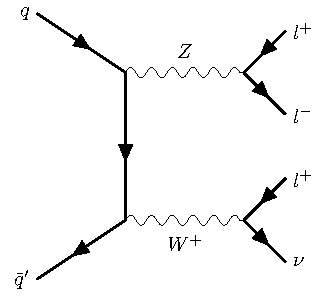
\includegraphics[width=\textwidth]{ubonn-thesis/Chapters/Chapters_04/Figure/Feynman_WZ.pdf}
    \caption{}
    \label{WZ}
  \end{subfigure}%% 
  \begin{subfigure}[b]{0.3\linewidth}
    \centering
    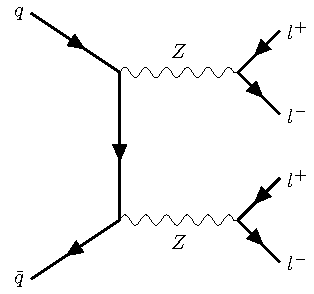
\includegraphics[width=\textwidth]{ubonn-thesis/Chapters/Chapters_04/Figure/Feynman_ZZ.pdf} 
    \caption{}
    \label{ZZ}
  \end{subfigure} 
  \begin{subfigure}[b]{0.3\linewidth}
    \centering
    \vspace*{-2.8cm}
    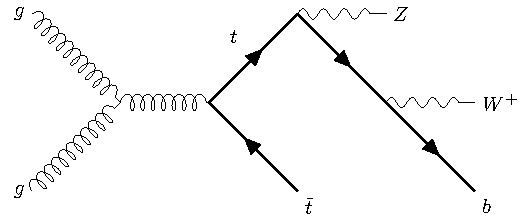
\includegraphics[width=\textwidth]{ubonn-thesis/Chapters/Chapters_04/Figure/tWZ_Feynman.pdf} 
    \caption{}
    \label{tWZ}
  \end{subfigure}%%
  \newline
  \begin{subfigure}[b]{0.3\linewidth}
    \centering
    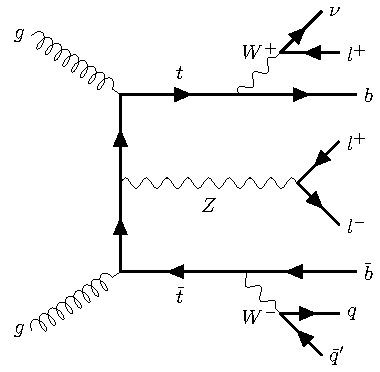
\includegraphics[width=0.9\textwidth]{ubonn-thesis/Chapters/Chapters_04/Figure/Feynman_ttbarV.pdf} 
    \caption{}
    \label{ttZ}
  \end{subfigure} 
  \begin{subfigure}[b]{0.3\linewidth}
    \centering
    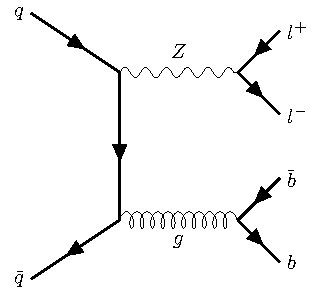
\includegraphics[width=0.9\textwidth]{ubonn-thesis/Chapters/Chapters_04/Figure/ZPlusJets_standalone.pdf} 
    \caption{}
    \label{Z+jets}
  \end{subfigure} 
  \begin{subfigure}[b]{0.3\linewidth}
    \centering
    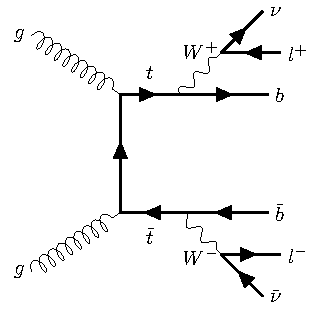
\includegraphics[width=0.9\textwidth]{ubonn-thesis/Chapters/Chapters_04/Figure/ttbar_standalone.pdf} 
    \caption{}
    \label{ttbar}
  \end{subfigure} 
  \caption{The leading order Feynman diagrams of the dominant background processes. (a) Diboson (WZ), (b) Diboson (ZZ), (c) tWZ, (d) $t\Bar{t}Z$, (e) Z+jets, and (f) $t\Bar{t}$}
  \label{background_feynman}
\end{figure}


Details of all simulated samples are given in table \ref{tab:backgrounds}.

\begin{table}[!h]
     \centering
      \begin{tabular}{@{} *6l  @{}}
      \toprule
      Process & MC generator & Parton shower & PDF set \\
     \midrule
      WZ & SHERPA 2.2.2 \cite{sherpa12004,sherpa2009} & SHERPA  & NNPDF3.0NNLO  \\[0.2ex] 
      ZZ & SHERPA 2.2.2 & SHERPA & NNPDF3.0NNLO  \\[0.2ex]
      $t\Bar{t}$ & POWHEG \cite{powhegOleari:2010nx} & Pythia 8 \cite{pythia2006} & NNPDF2.3LO  \\[0.2ex]
      tW & POWHEG & Pythia 8 & NNPDF2.3LO  \\[0.2ex]
      Z+jets & SHERPA 2.2.1 & SHERPA & NNPDF3.0NNLO  \\[0.2ex]
      $t\Bar{t}V$ & MadGraph5$\_$aMC@NLO & Pythia 8 \cite{pythia82015}&  NNPDF2.3LO  \\[0.2ex]
      tWZ & MadGraph5$\_$aMC@NLO & Pythia 8 &  NNPDF2.3LO  \\[0.2ex]
      $t\Bar{t}H$ & POWHEG  & Pythia 8 &  NNPDF2.3LO  \\[0.2ex]
      \bottomrule
 \end{tabular}
 \caption{Overview of background MC generated samples.}
 \label{tab:backgrounds}
 \end{table}

\newpage

\subsection{Reweighting of Monte-Carlo simulated events}
\label{subsec:reweightingofMC}
The number of events generated during the MC simulations generally do not exactly match the number of expected events for a given physical process at a given integrated luminosity. Each MC event is given a weight to rescale it so that the overall MC sample accurately represents the physical processes. Thus, to correctly reproduce the data-taking conditions, as well as replicate the efficiency of selecting different physics objects, in the simulated samples, event-by-event correction factors are applied to the MC events. The total event weight can be written as:
\begin{equation}
    \label{eqn:weight}
    w_{event} = w_{MC}\times w_{pile-up} \times w_{lepton} \times w_{JVT} \times w_{trigger} \times w_{b-tagging}
\end{equation}

The term $ w_{MC}$ is the MC event weight. The $ w_{pile-up}$ term is introduced to the MC samples, as a certain pile-up profile is assumed during MC simulation where as  $ w_{lepton}$ term is related to the efficiency of reconstructing, identifying a certain lepton. The $ w_{trigger}$ term is realted to the trigger. The final state considered for analysis consists of a  b-tagged jet, thus   $ w_{b-tagging}$ weight is applied.

\subsection{Luminosity reweighting}
\label{subsec:luminosityreweighting}

\begin{figure}[!h]
\centering
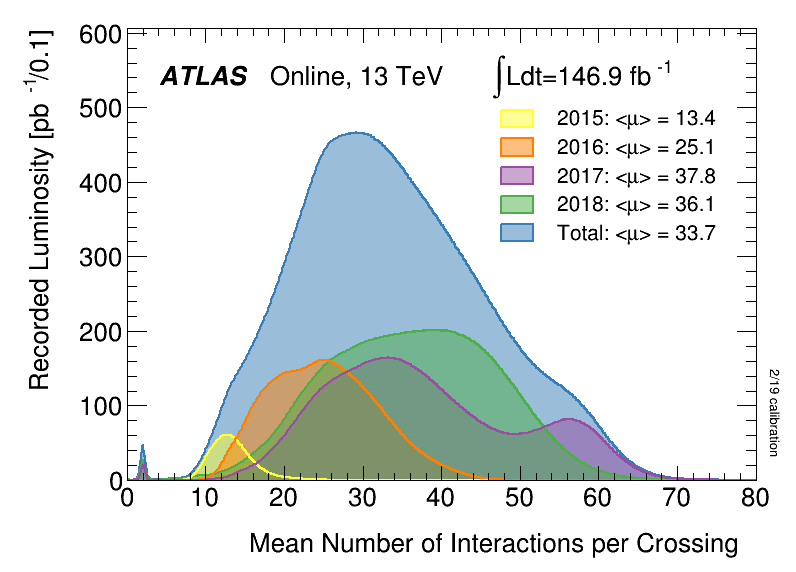
\includegraphics[width=0.5\textwidth]{ubonn-thesis/Chapters/Chapters_04/Figure/mu_2015_2018.png}
\caption{Luminosity weighted plot of the mean number of interactions per crossing for the 2015 and 2016 datasets \cite{ATLAS-CONF-2020-023}.}
\label{}
\end{figure}


The signal and background processes are simulated with large statistics. Thus, the luminosity for the MC simulated samples are very high. In order to correctly match the process to a dataset, the luminosity of the MC sample is scaled. The weight or scale factor is defined as 

\begin{equation}
    \label{luminosity}
    w_{lumi} = \frac{\sigma_{process}}{N} \mathcal{L}
\end{equation}

$\sigma_{process}$ is the cross-section of the specific physical process. $\mathcal{L}$ is the integrated luminosity of the data sample and N is the number of events in the original MC sample.
